\section{Results}

\subsection{Variation in observed hospital thrombolysis use}

Thrombolysis use in the original data varied between hospitals from 1.5\% to 24.3\% of all patients, and 7.3\% to 49.7\% of patients arriving within 4 hours of known (precise or estimated) stroke onset.

%%%%%%%%%%%%%%%%%%%%%%%%%%%%%%%%%%%%%%%%%%%%%%%%%%%%%%%%%%%%%%%%%%%%%%%%

\subsection{Feature selection}

The best model with 1, 2, 5, 10, 25 \& all 60 original features had ROC AUCs of 0.715, 0.792, 0.891, 0.919, 0.923 \& 0.922. We selected 10 features for all subsequent work, which were:

\begin{itemize}
    \item \emph{Arrival-to-scan time}: Time from arrival at hospital to scan (mins)
    \item \emph{Infarction}: Stroke type (1 = infarction, 0 = haemorrhage)
    \item \emph{Stroke severity}: National Institutes of Health Stroke Scale (NIHSS) score on arrival
    \item \emph{Precise onset time}: Onset time (1 = precise, 0 = best estimate)
    \item \emph{Prior disability level}: Disability level (modified Rankin Scale; mRS) before stroke
    \item \emph{Stroke team}: Stroke team attended (hospital identifier)
    \item \emph{Use of anticoagulants}: Use of prior anticoagulant (1 = Yes, 0 = No)
    \item \emph{Onset-to-arrival time}: Time from onset of stroke to arrival at hospital (mins)
    \item \emph{Onset during sleep}: Did stroke occur in sleep?
    \item \emph{Age}: Age (as midpoint of 5 year age bands)
\end{itemize}

These were not necessarily the 10 most important features, as another highly correlated feature may also have been important, but if a feature is highly correlated with an already chosen feature, it will add less additional value.

Correlations between the 10 features were measured using coefficients of determination (r-squared). All r-squared were less than 0.05 except a) age and prior disability level (r-squared 0.146), and b) onset during sleep and precise onset time (r-squared 0.078).

%%%%%%%%%%%%%%%%%%%%%%%%%%%%%%%%%%%%%%%%%%%%%%%%%%%%%%%%%%%%%%%%%%%%%%%%

\subsubsection{Model accuracy}

Should be contrasted to the original model already published.  The point is that you've got a nice explainable model here with very similar accuracy.  Make that clear.

Model accuracy was measured using stratified 5-fold cross validation. Overall accuracy was 85.0\% (83.9\% sensitivity and specificity could be achieved simultaneously). The ROC AUC was 0.918. The model predicted hospital thrombolysis use at each hospital with very good accuracy (r-squared = 0.977).

The appendix contains further model accuracy analysis (including patient subgroup analysis).

%%%%%%%%%%%%%%%%%%%%%%%%%%%%%%%%%%%%%%%%%%%%%%%%%%%%%%%%%%%%%%%%%%%%%%%%
\subsection{Individual patient SHAP values}
SHAP values are presented as how they affect log odds of receiving thrombolysis, but for individual predictions, probability values are more intuitive. Figure \ref{fig:results_waterfall} shows waterfall plots for an example of a patient with low (top) and high (bottom) probability of receiving thrombolysis. Waterfall plots show the influence of features for an individual prediction (in our case, patient). The SHAP model starts with a base prediction of a 24\% probability of receiving thrombolysis, before feature values are taken into account. For the patient with a low probability of receiving thrombolysis, the two most influential features reducing the probability of receiving thrombolysis were a long arrival-to-scan time (138 minutes) and a low stroke severity (NIHSS=2). For the patient with a high probability of receiving thrombolysis, the two most influential features increasing the probability of receiving thrombolysis were a short arrival-to-scan time (17 minutes) and a moderate stroke severity (NIHSS=14). 

\begin{figure}[!h]
\centering
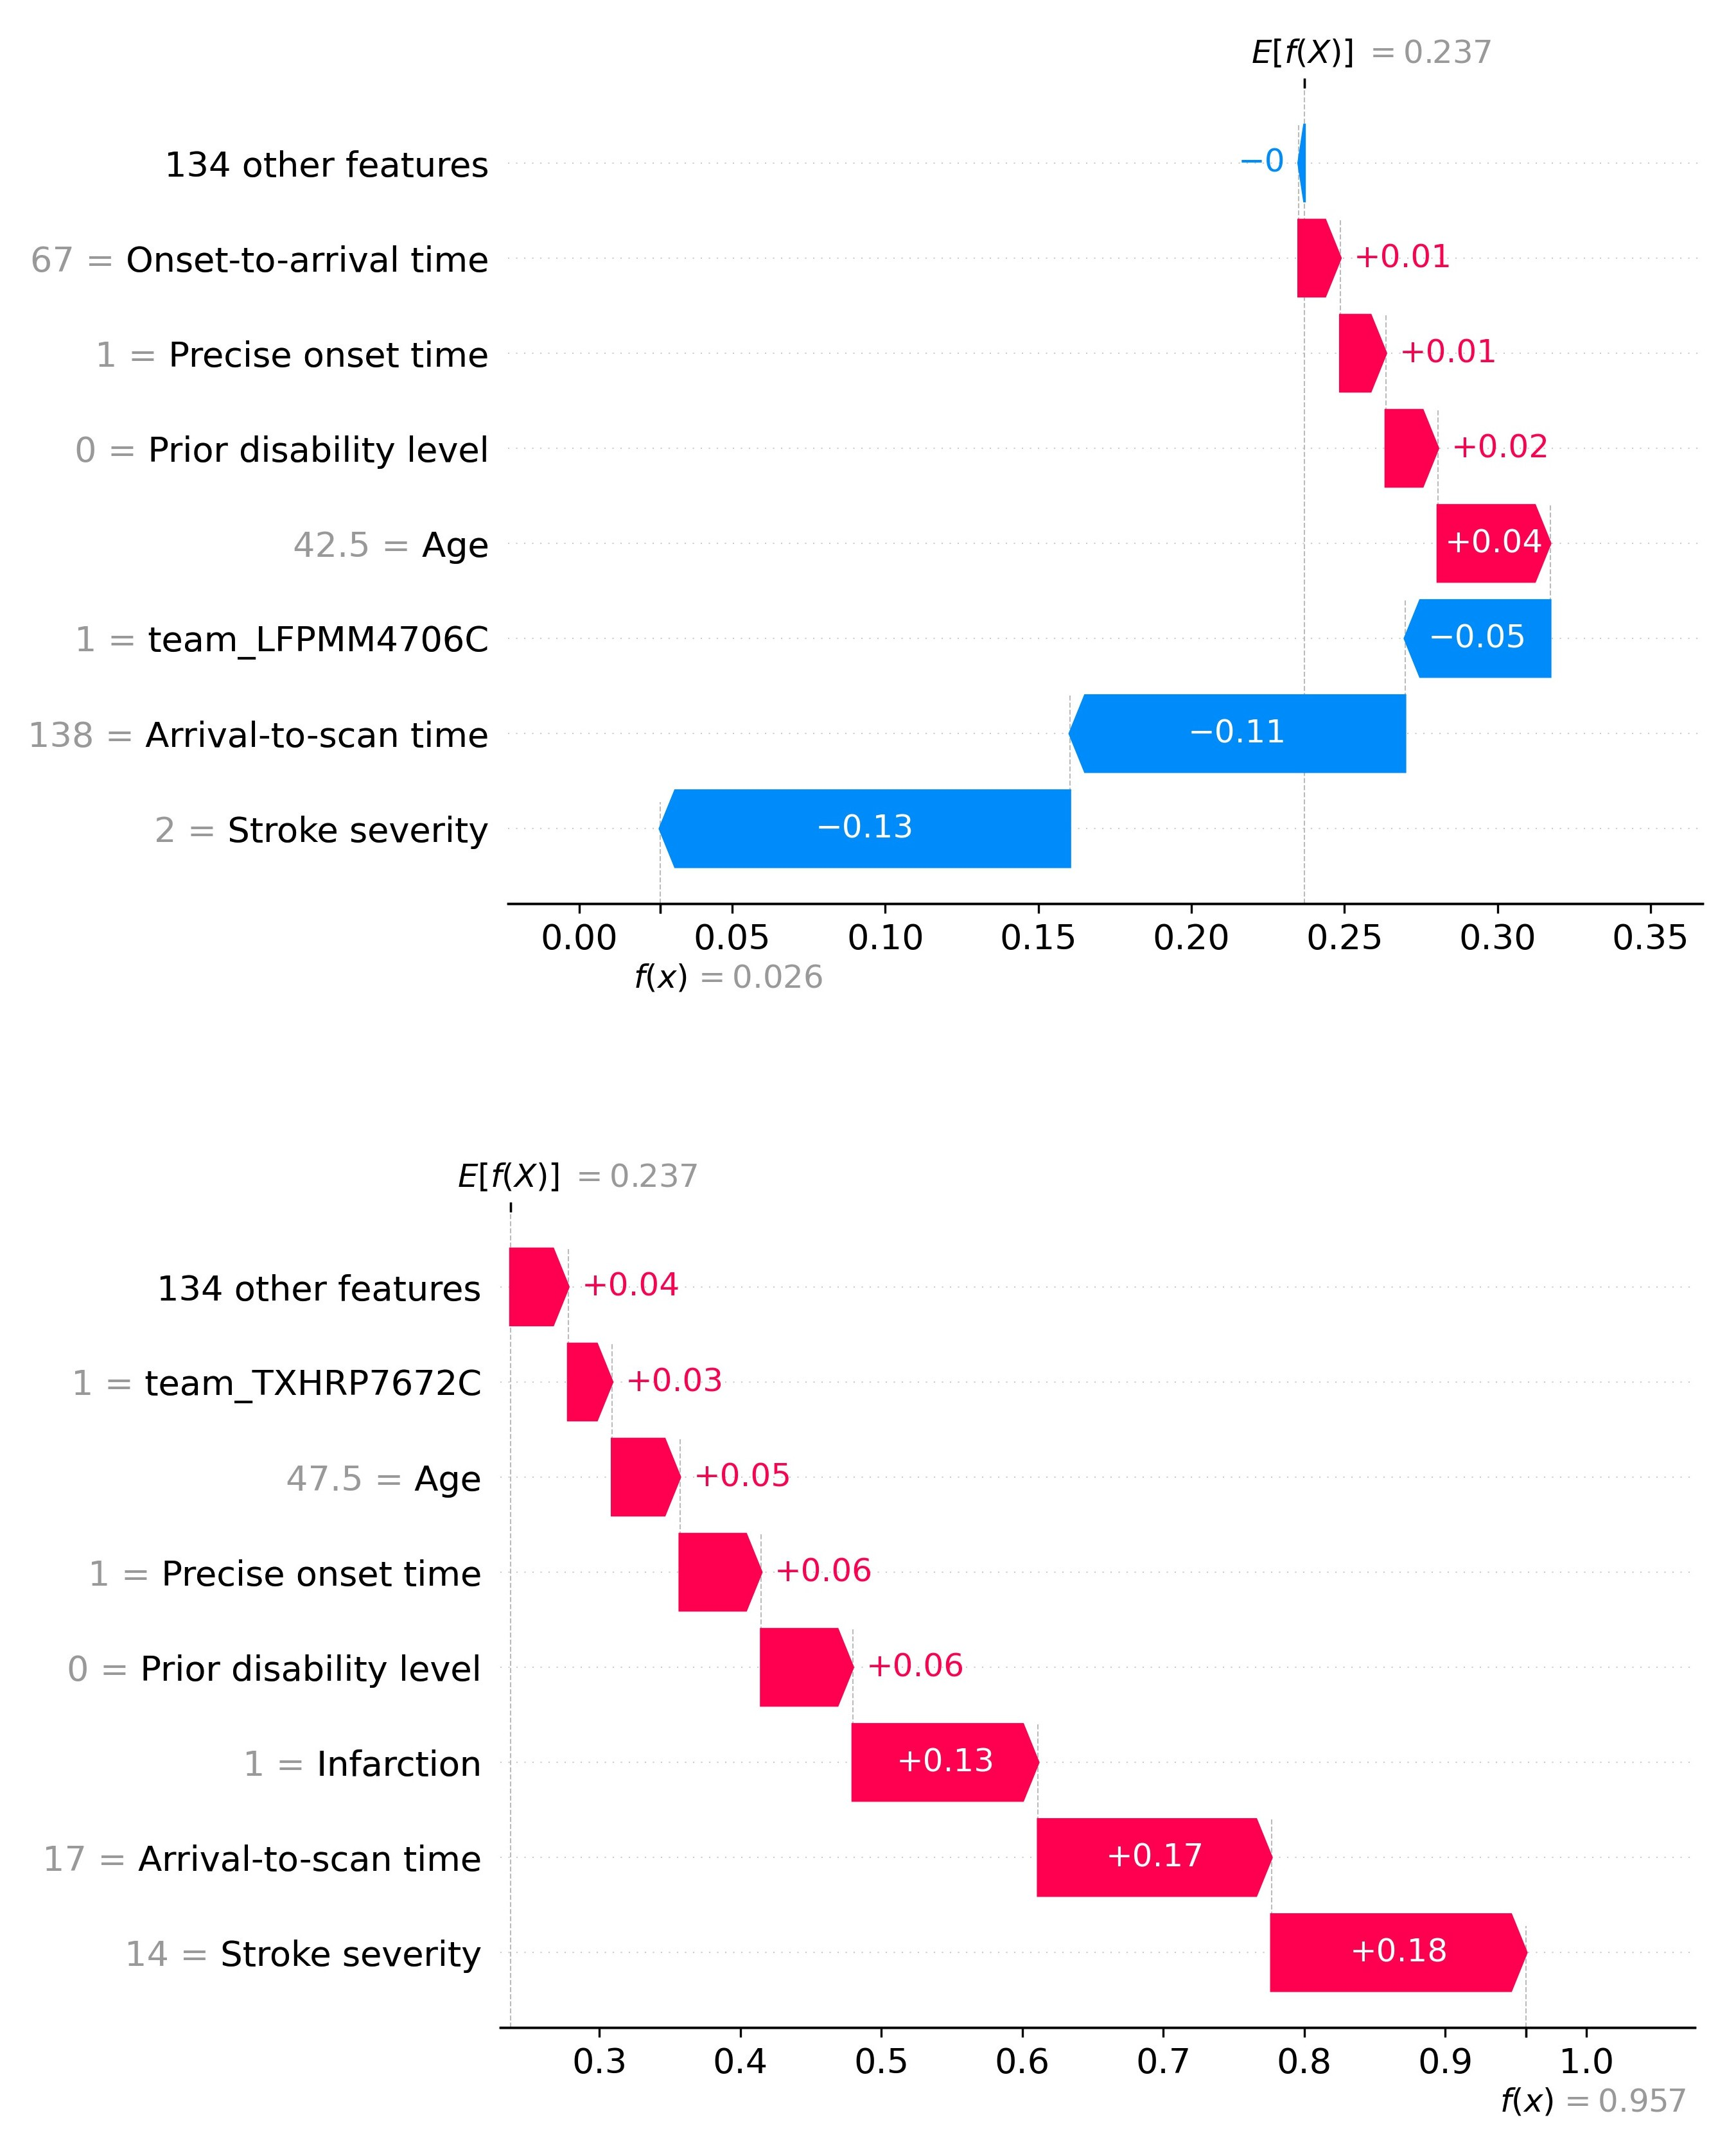
\includegraphics[width=0.6\textwidth]{./images/waterfall}
\caption{Waterfall plots showing the influence of each feature on the predicted probability of a single patient receiving thrombolysis. Top: An example of a patient with a low probability (2.6\%) of receiving thrombolysis. Bottom: An example of a patient with a high probability (95.7\%) of receiving thrombolysis.}
\label{fig:results_waterfall}
\end{figure}

%\newpage
%%%%%%%%%%%%%%%%%%%%%%%%%%%%%%%%%%%%%%%%%%%%%%%%%%%%%%%%%%%%%%%%%%%%%%%%

\subsection{The relationship between feature values and the odds of receiving thrombolysis}

Figure \ref{fig:shap_feature_subfigure_a} shows the relationship between patient feature values and SHAP values. Figure \ref{fig:shap_feature_subfigure_b} shows the range of SHAP values for the one-hot encoded hospital feature. Key observations are (with SHAP influence converted from log-odds to odds):

\begin{itemize}
    \item \emph{Stroke type}: The SHAP values for stroke type show that the model effectively eliminated any probability of receiving thrombolysis for non-ischaemic (haemorrhagic) stroke, with the odds of receiving thrombolysis fell by over 7,000 fold.
    \item \emph{Arrival-to-scan time}: The odds of receiving thrombolysis reduced by about 9 fold over the first 120 minutes of arrival to scan time.
    \item \emph{Stroke severity (NIHSS)}: The odds of receiving thrombolysis were lowest at NIHSS 0, increased and peaked at NIHSS 15-25, and then fell again with higher stroke severity (NIHSS above 25). The difference between minimum odds (at NIHSS 0) and maximum odds (at 15-25) of receiving thrombolysis was about 30 fold.
    \item \emph{Stroke onset time type (precise vs. estimated)}: The odds of receiving thrombolysis were about 3 fold greater for precise onset time than estimated onset time.
    \item \emph{Disability level (mRS) before stroke}: The odds of receiving thrombolysis fell about 6 fold between mRS 0 and 5.
    \item \emph{Use of AF anticoagulants}: The odds of receiving thrombolysis were about 5 fold greater for no use.
    \item \emph{Onset-to-arrival time}: The odds of receiving thrombolysis were similar below 120 minutes, then fell about 3 fold above 120.
    \item \emph{Age}: The odds of receiving thrombolysis were similar below 80 years old, then fell about 1.8 fold between 80 and 110 years old.    
    \item \emph{Onset during sleep}: The odds of receiving thrombolysis were about 4 fold lower for onset during sleep.
    \item \emph{Hospital attended}: There was a 13 fold difference in odds of receiving thrombolysis between hospitals.
\end{itemize}

In summary the most thrombolysable patients have:
\begin{itemize}
    \item an infarction stroke type
    \item shorter arrival-to-scan times
    \item moderate to severe stroke severity with NIHSS 5-25
    \item a precise onset time
    \item lower pre-stroke disability
    \item were not taking anticoagulant medication
    \item shorter onset-to-arrival times
    \item were younger
    \item did not have onset during sleep
    \item a better chance of receiving thrombolysis at certain hospitals
\end{itemize}
%\newpage

\begin{figure}%[!h]
\centering
\begin{subfigure}{.9\textwidth}
  \centering
    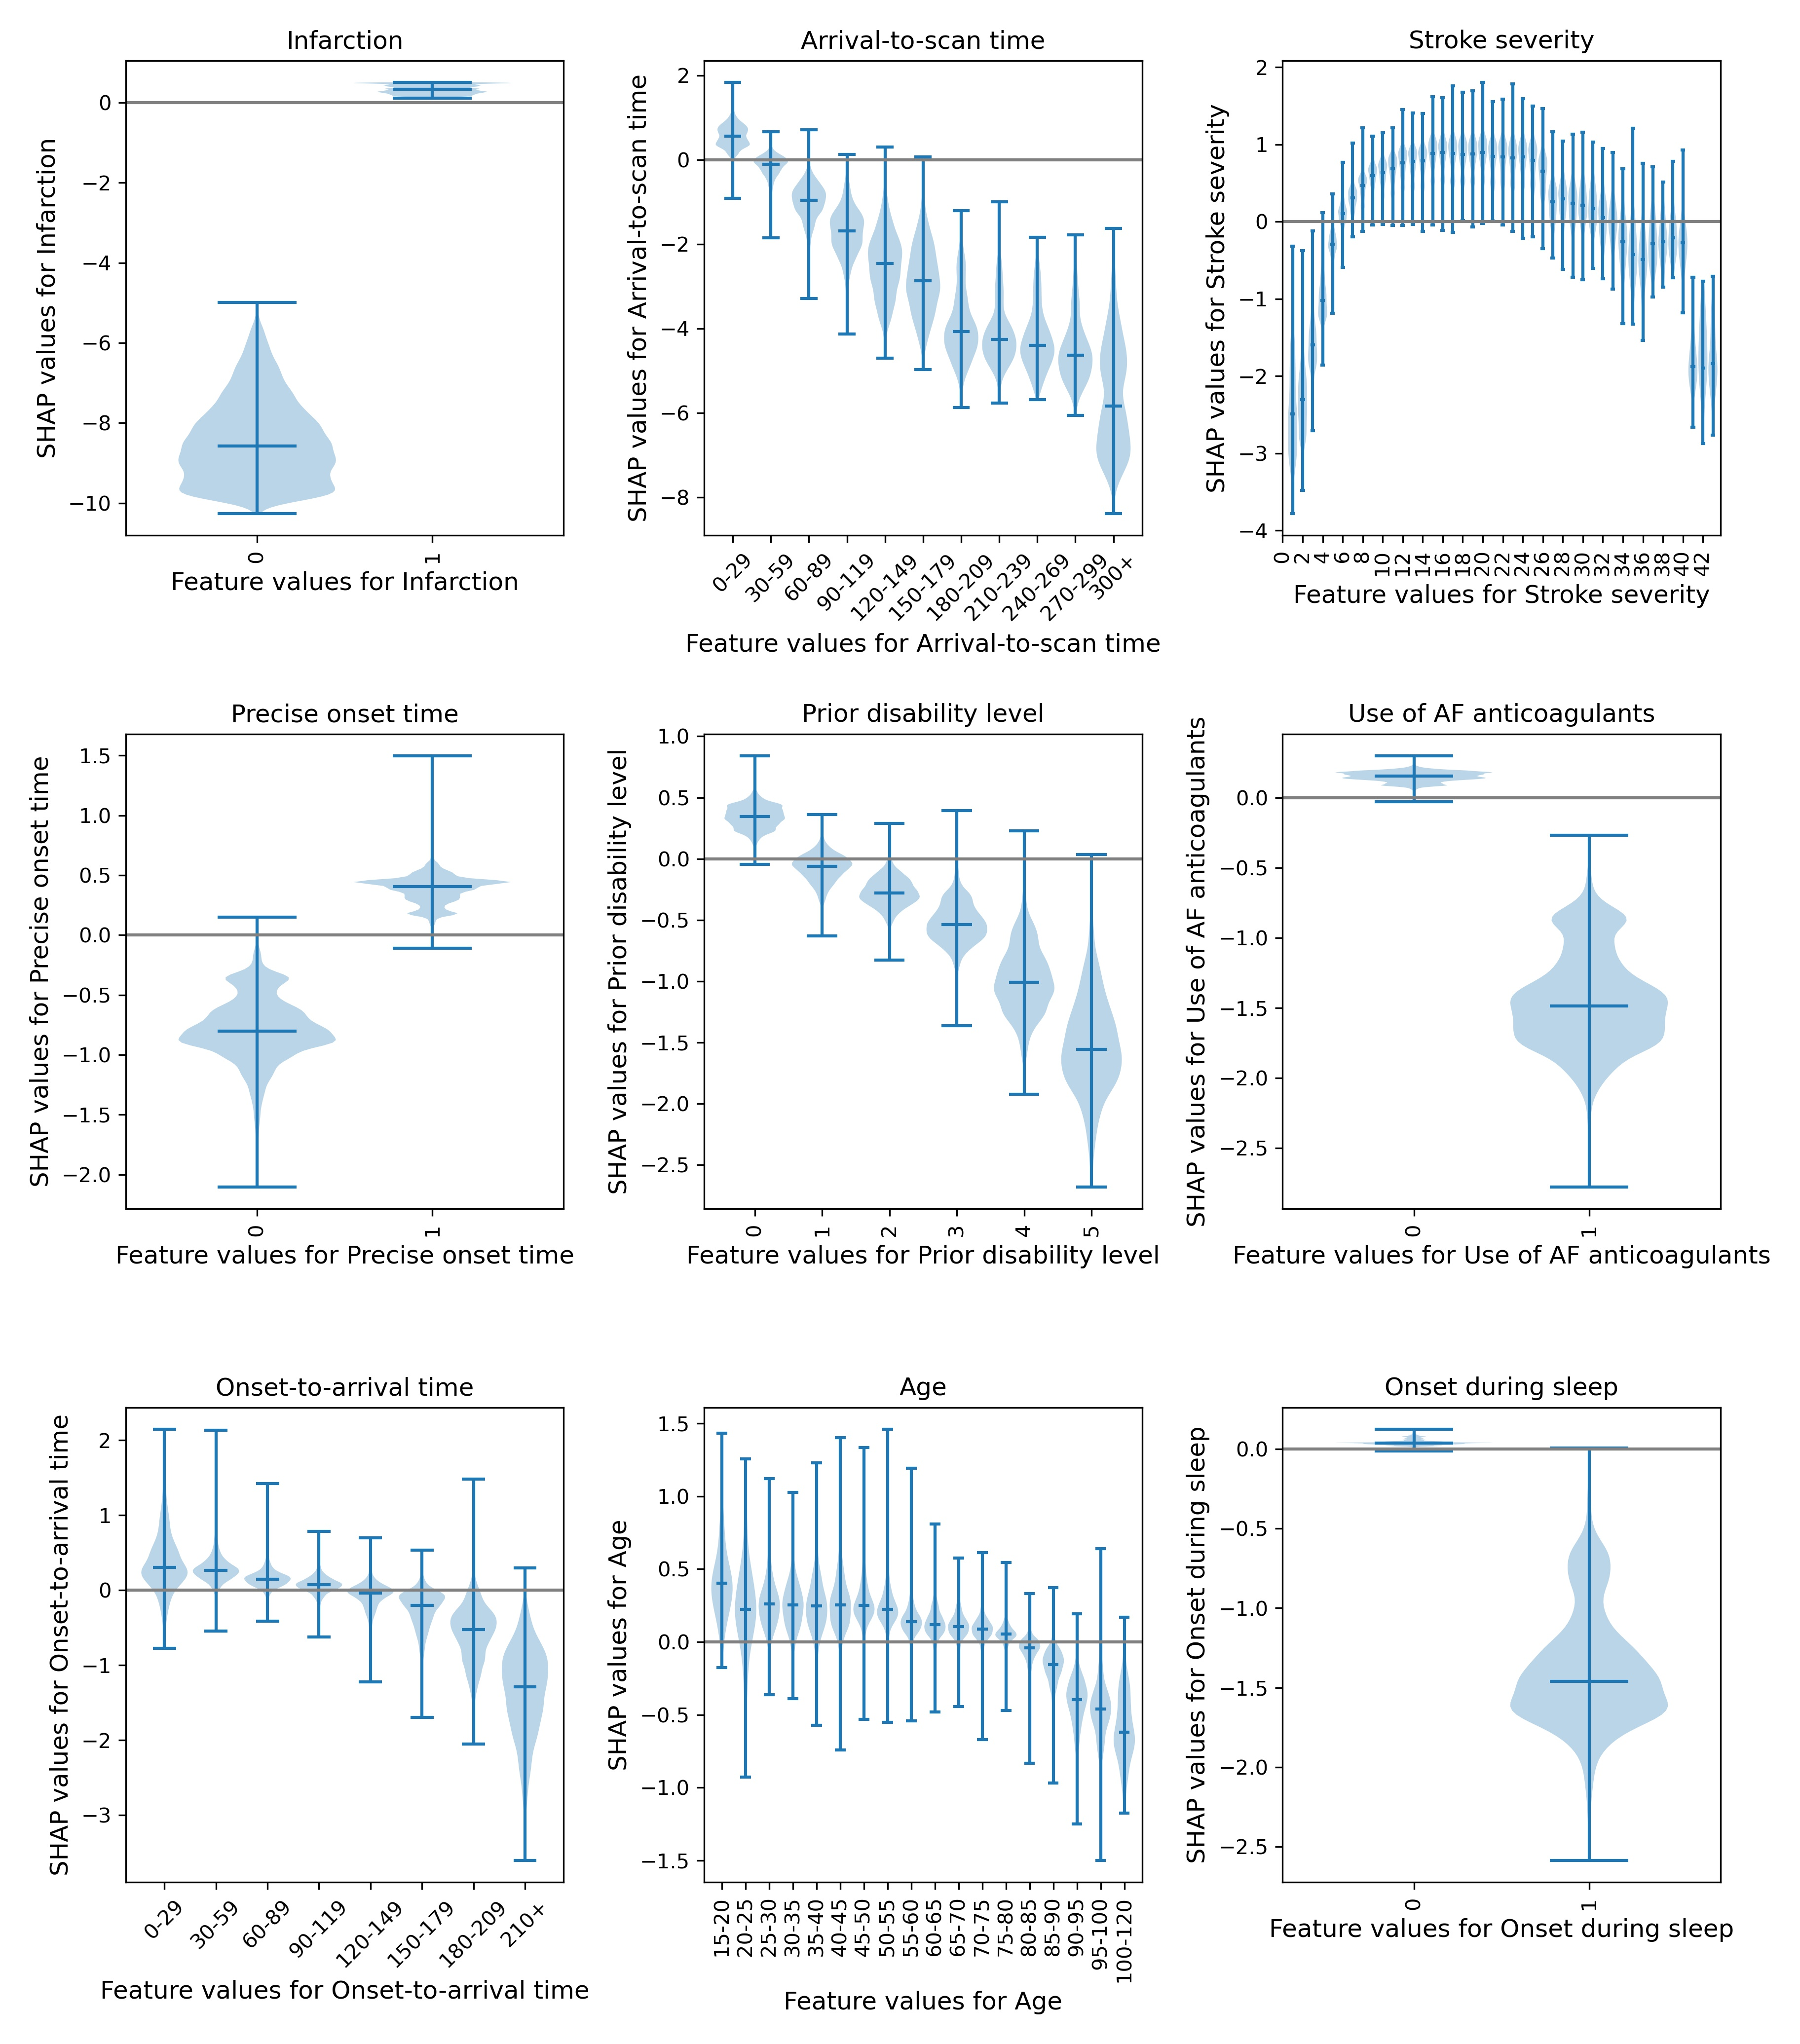
\includegraphics[width=1.\textwidth]{./images/03d_xgb_10_features_thrombolysis_shap_violin_all_features}
    \caption{}
  \label{fig:shap_feature_subfigure_a}
\end{subfigure}
\begin{subfigure}{.9\textwidth}
  \centering
    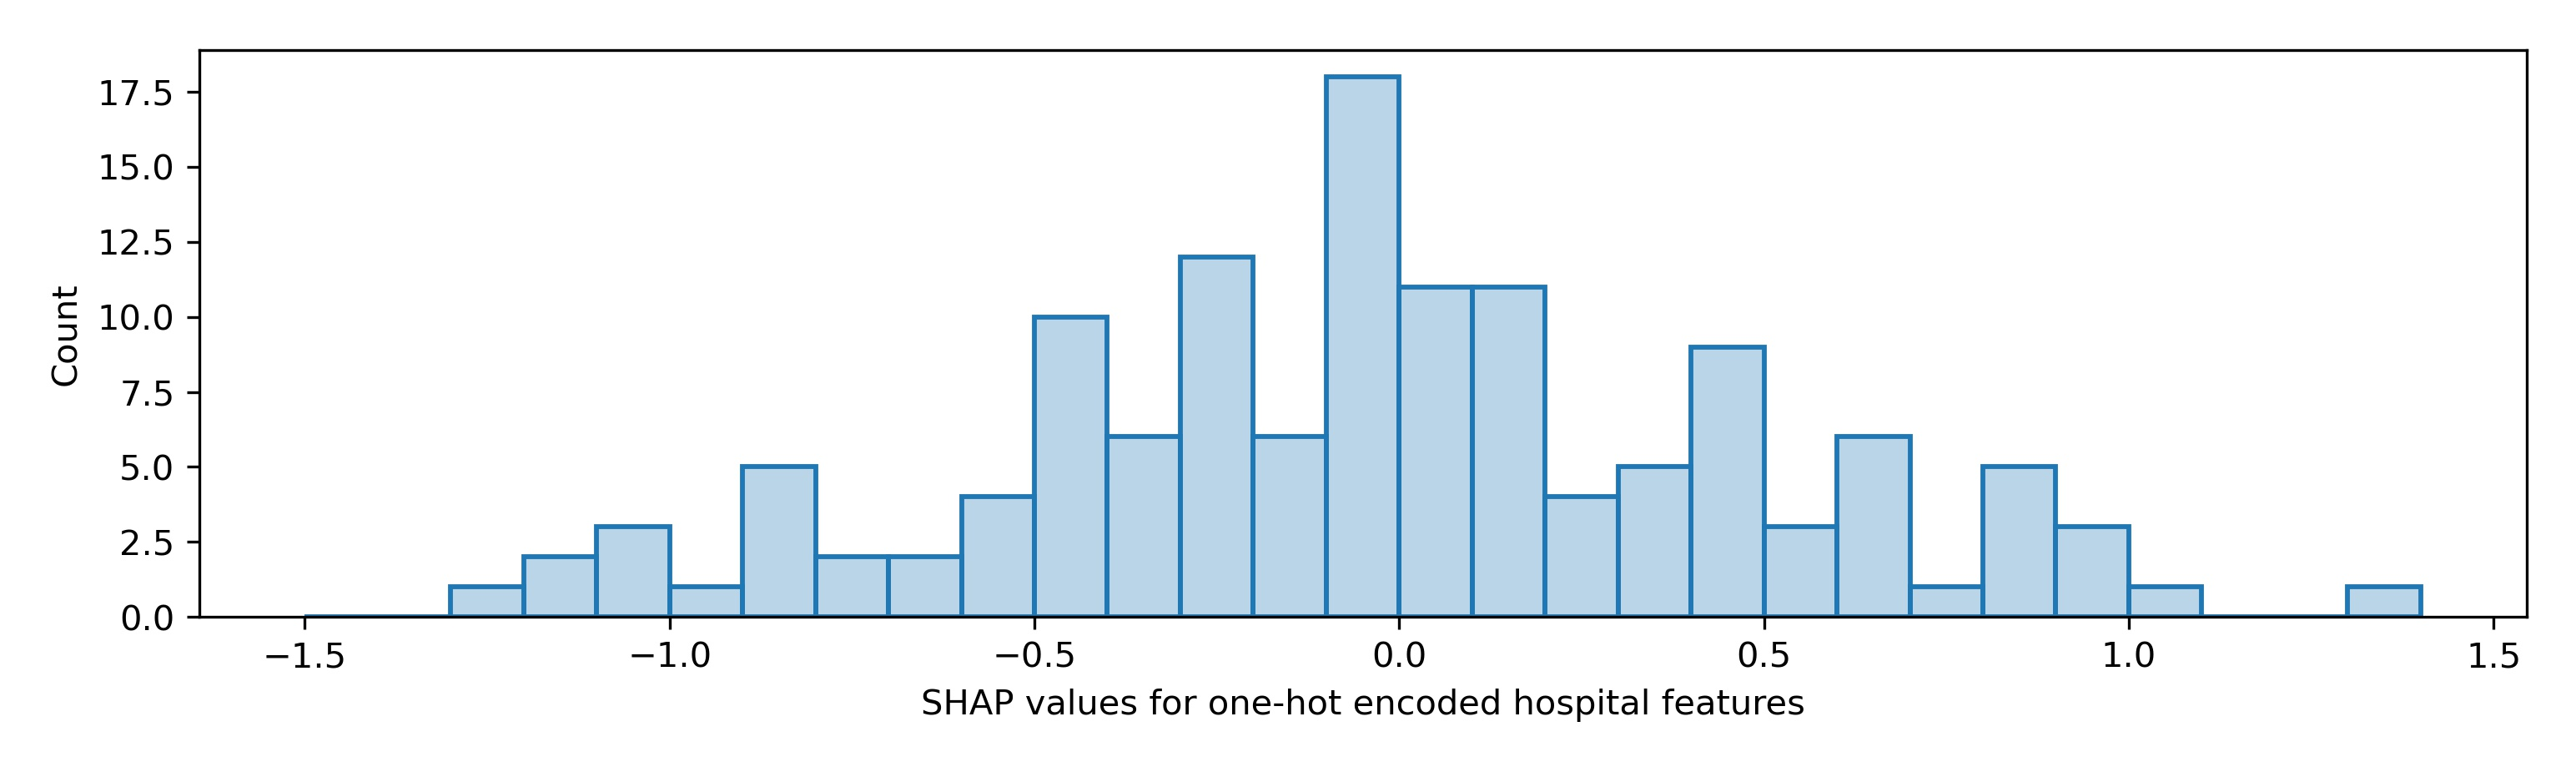
\includegraphics[width=1.\textwidth]{./images/03d_xgb_10_features_hosp_shap_hist}
    \caption{}
  \label{fig:shap_feature_subfigure_b}
\end{subfigure}
\caption{(a) Violin plots showing the relationship between SHAP values and feature values. The horizontal line shows the median SHAP value. The plots are ordered in ranked feature importance (using the mean absolute SHAP value across all instances) (b) Histogram showing the frequency of SHAP values for the one-hot encoded hospital feature.}
%\label{fig:shap_correlation_subfigure}
\end{figure}

%%%%%%%%%%%%%%%%%%%%%%%%%%%%%%%%%%%%%%%%%%%%%%%%%%%%%%%%%%%%%%%%%%%%%%%%
%\newpage
\subsection{How the hospital SHAP value compares with the hospitals use of thrombolysis}

The median hospital SHAP value correlated with the observed hospital thrombolysis rate with an r-squared of 0.582 (figure \ref{fig:shap_correlation_subfigure_a}), suggesting that 58\% (P$<$0.0001) of the between-hospital variance in thrombolysis use may be explained by the hospitals' SHAP values, i.e. the hospitals' predisposition and/or preparedness to use thrombolysis. By comparison, only four of the patient features had an r-squared greater than 0.1, P$<$0.0001 (infarction 0.448, arrival-to-scan time 0.273, anticoagulants 0.213, stroke severity 0.153), and with a maximum of 45\% of the between-hospital variance in thrombolysis use being explained by a single patient feature (infarction).

Using the \emph{10k holdout model}, the predicted use of thrombolysis across the 132 hospitals for the identical 10k cohort of patients (not used in training the model) ranged from 10\% to 45\%. The median hospital SHAP value for the 10k cohort of patients correlated very closely with the predicted thrombolysis use in the 10k cohort of patients at each hospital, with an r-squared of 0.944 (figure \ref{fig:shap_correlation_subfigure_b}), confirming that the hospital SHAP is providing a direct insight into a hospitals' propensity to use thrombolysis.

%\iffalse
\begin{figure}[!h]
\centering
\begin{subfigure}{.49\textwidth}
  \centering
    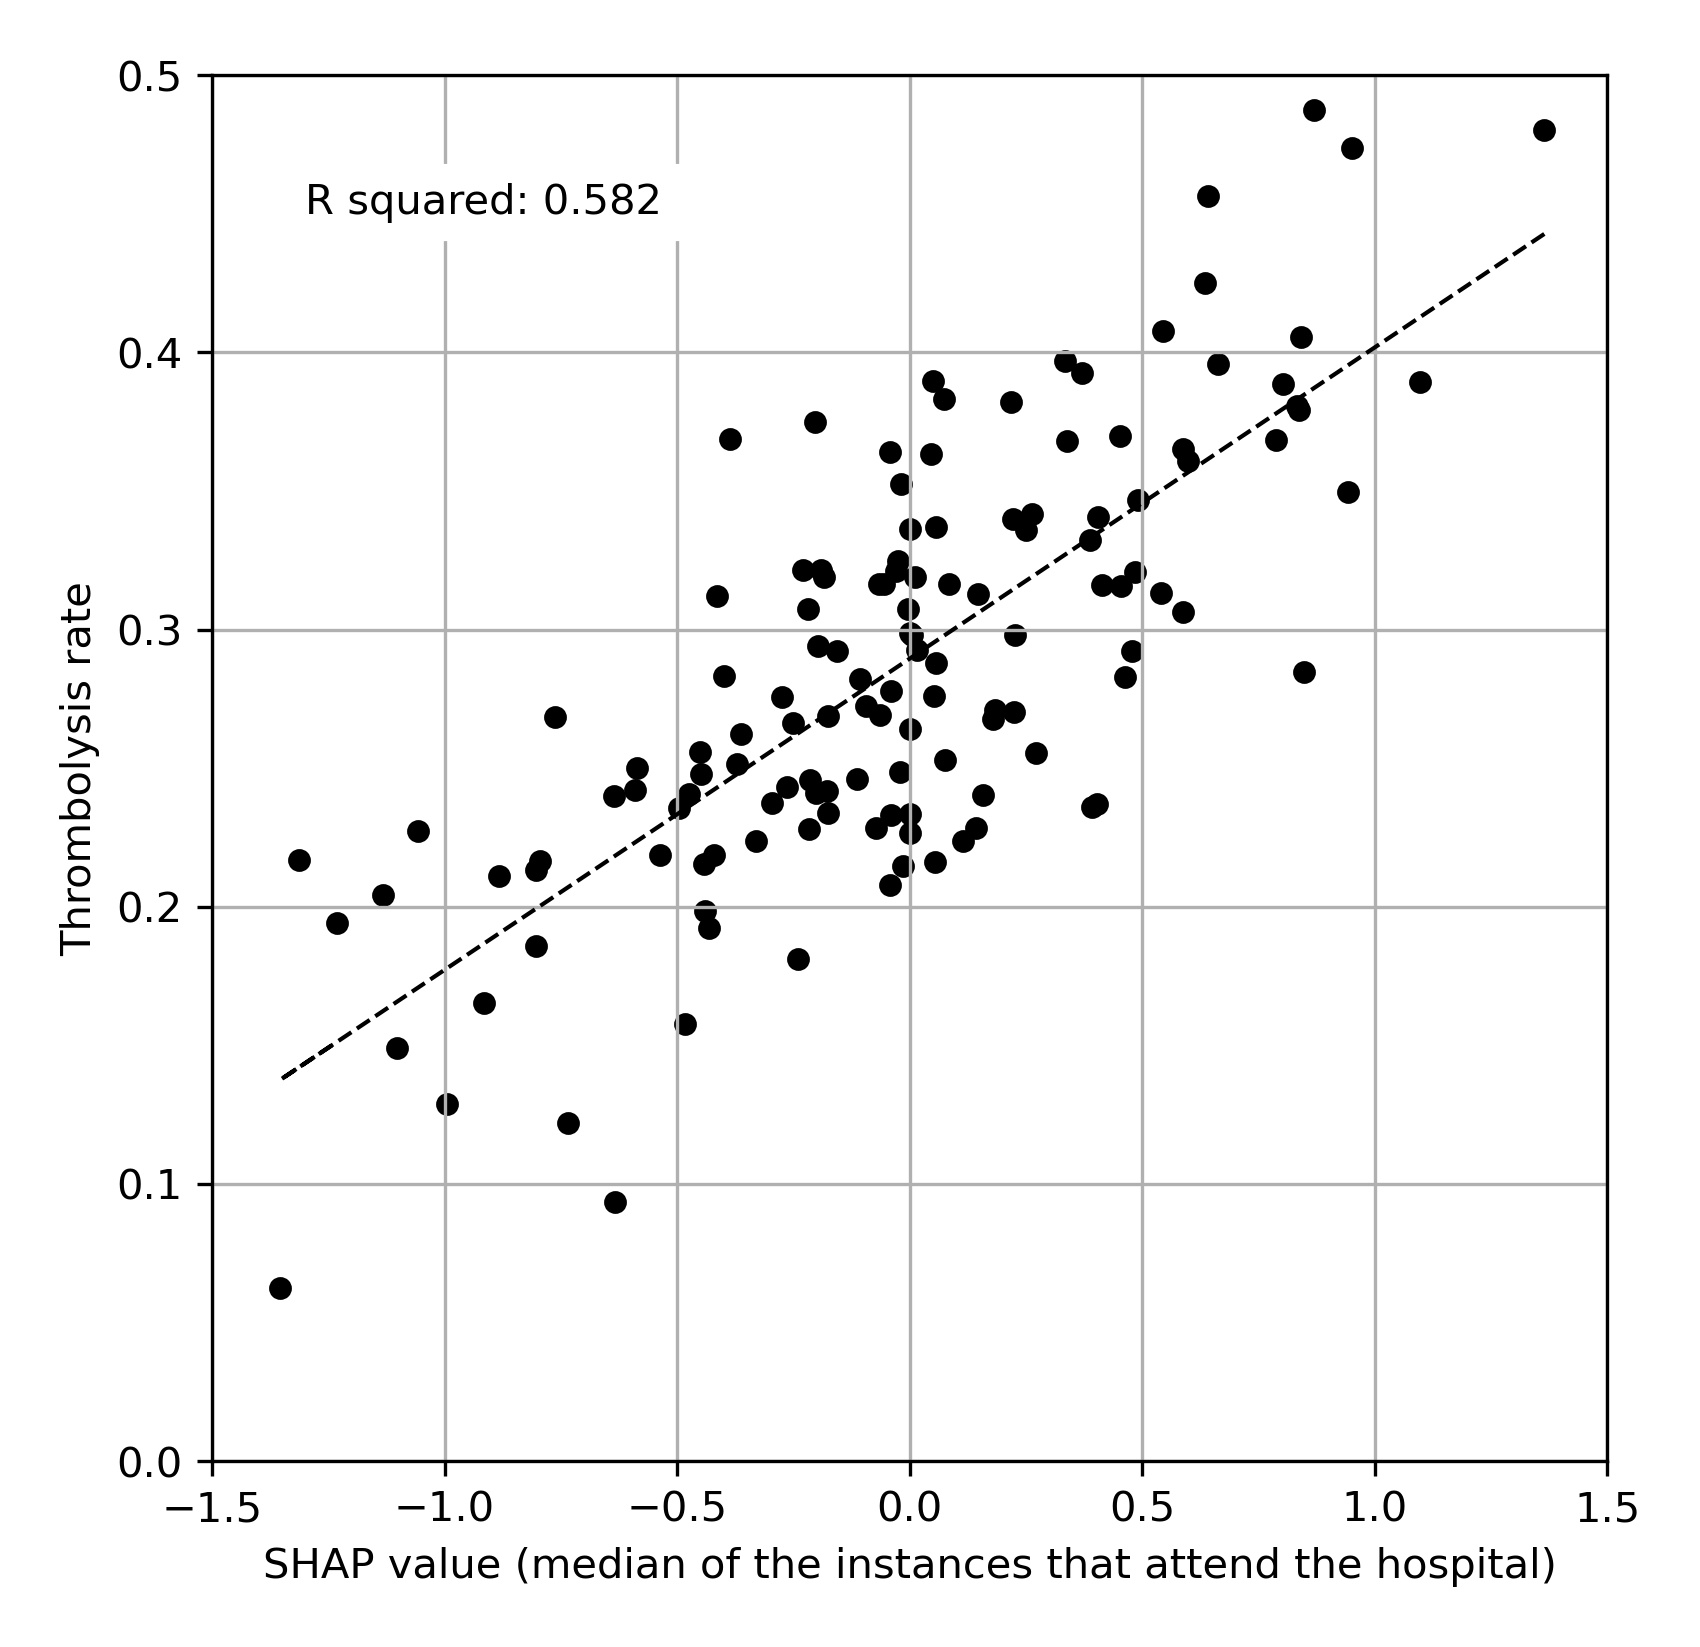
\includegraphics[width=0.9\textwidth]{./images/03c_xgb_10_features_attended_hosp_shap_value}
    \caption{}
  \label{fig:shap_correlation_subfigure_a}
\end{subfigure}
\begin{subfigure}{.49\textwidth}
  \centering
    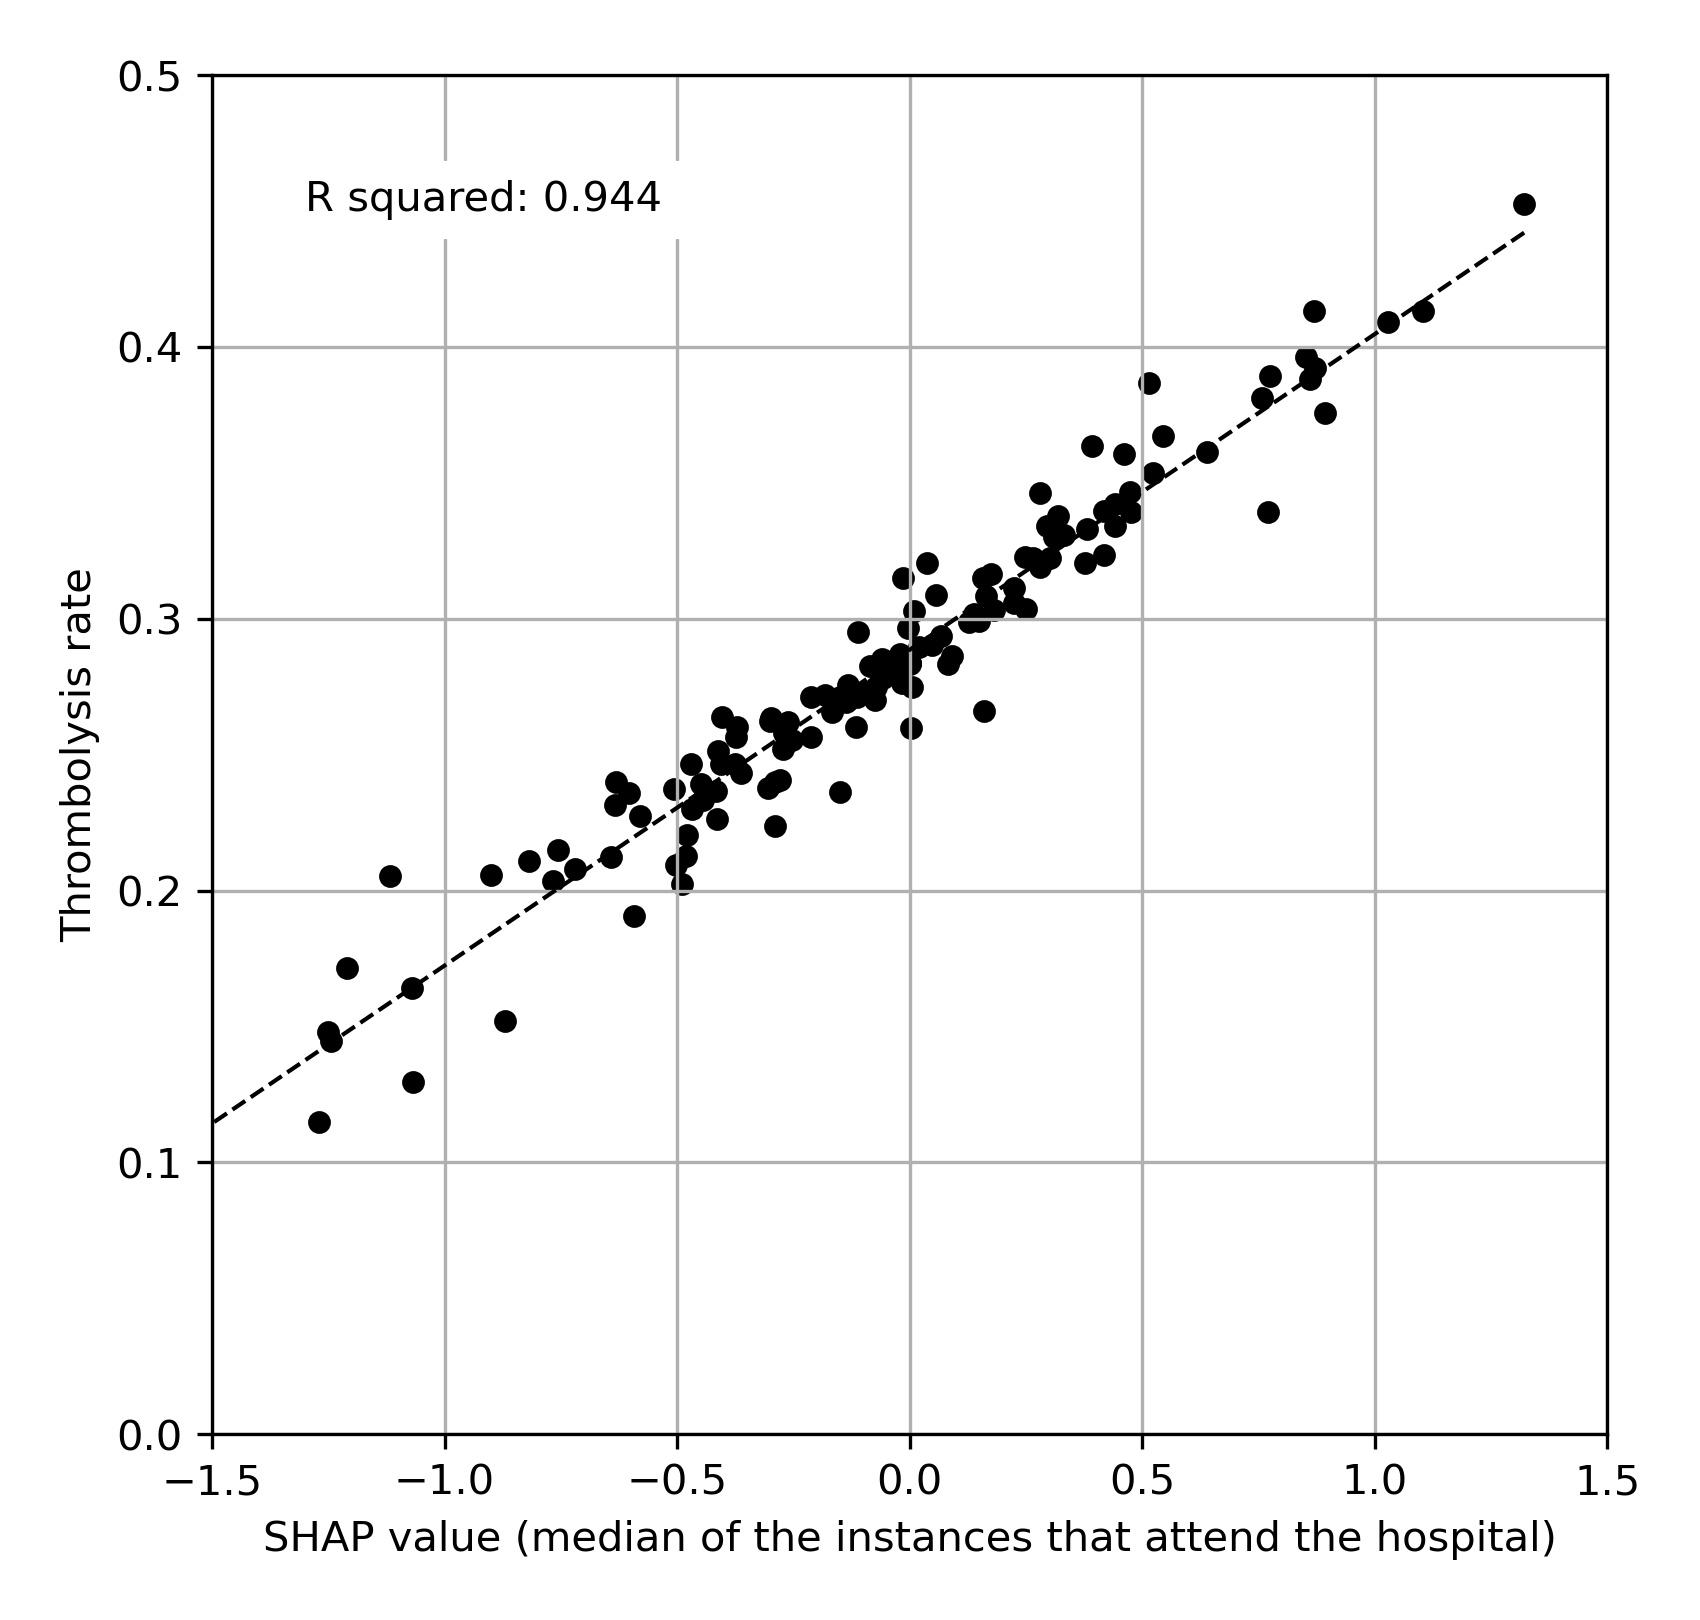
\includegraphics[width=0.9\textwidth]{./images/04_xgb_10_features_10k_cohort_attended_hosp_shap_value}
    \caption{}
  \label{fig:shap_correlation_subfigure_b}
\end{subfigure}
\caption{(a) Correlation between median hospital SHAP value and the observed thrombolysis use at each hospital. (b) Correlation between median hospital SHAP value and the predicted thrombolysis use at each hospital (using the 10k holdout model).}
%\label{fig:shap_correlation_subfigure}
\end{figure}
%%%%%%%%%%%%%%%%%%%%%%%%%%%%%%%%%%%%%%%%%%%%%%%%%%%%%%%%%%%%%%%%%%%
%\fi


%\newpage
\subsection{How much of the hospitals use of thrombolysis can be explained by the differences in the hospital processes, and the differences in the patient mix}

Figure \ref{fig:shap_multiple_regression} shows that 35\% of the variance in observed between-hosptial thrombolysis use can be explained by the patient mix, 72\% can be explained by hospital processes, and that 94\% can be explained by the combined information from both patient mix and hospital processes. 


\begin{figure}[!h]
    \centering
    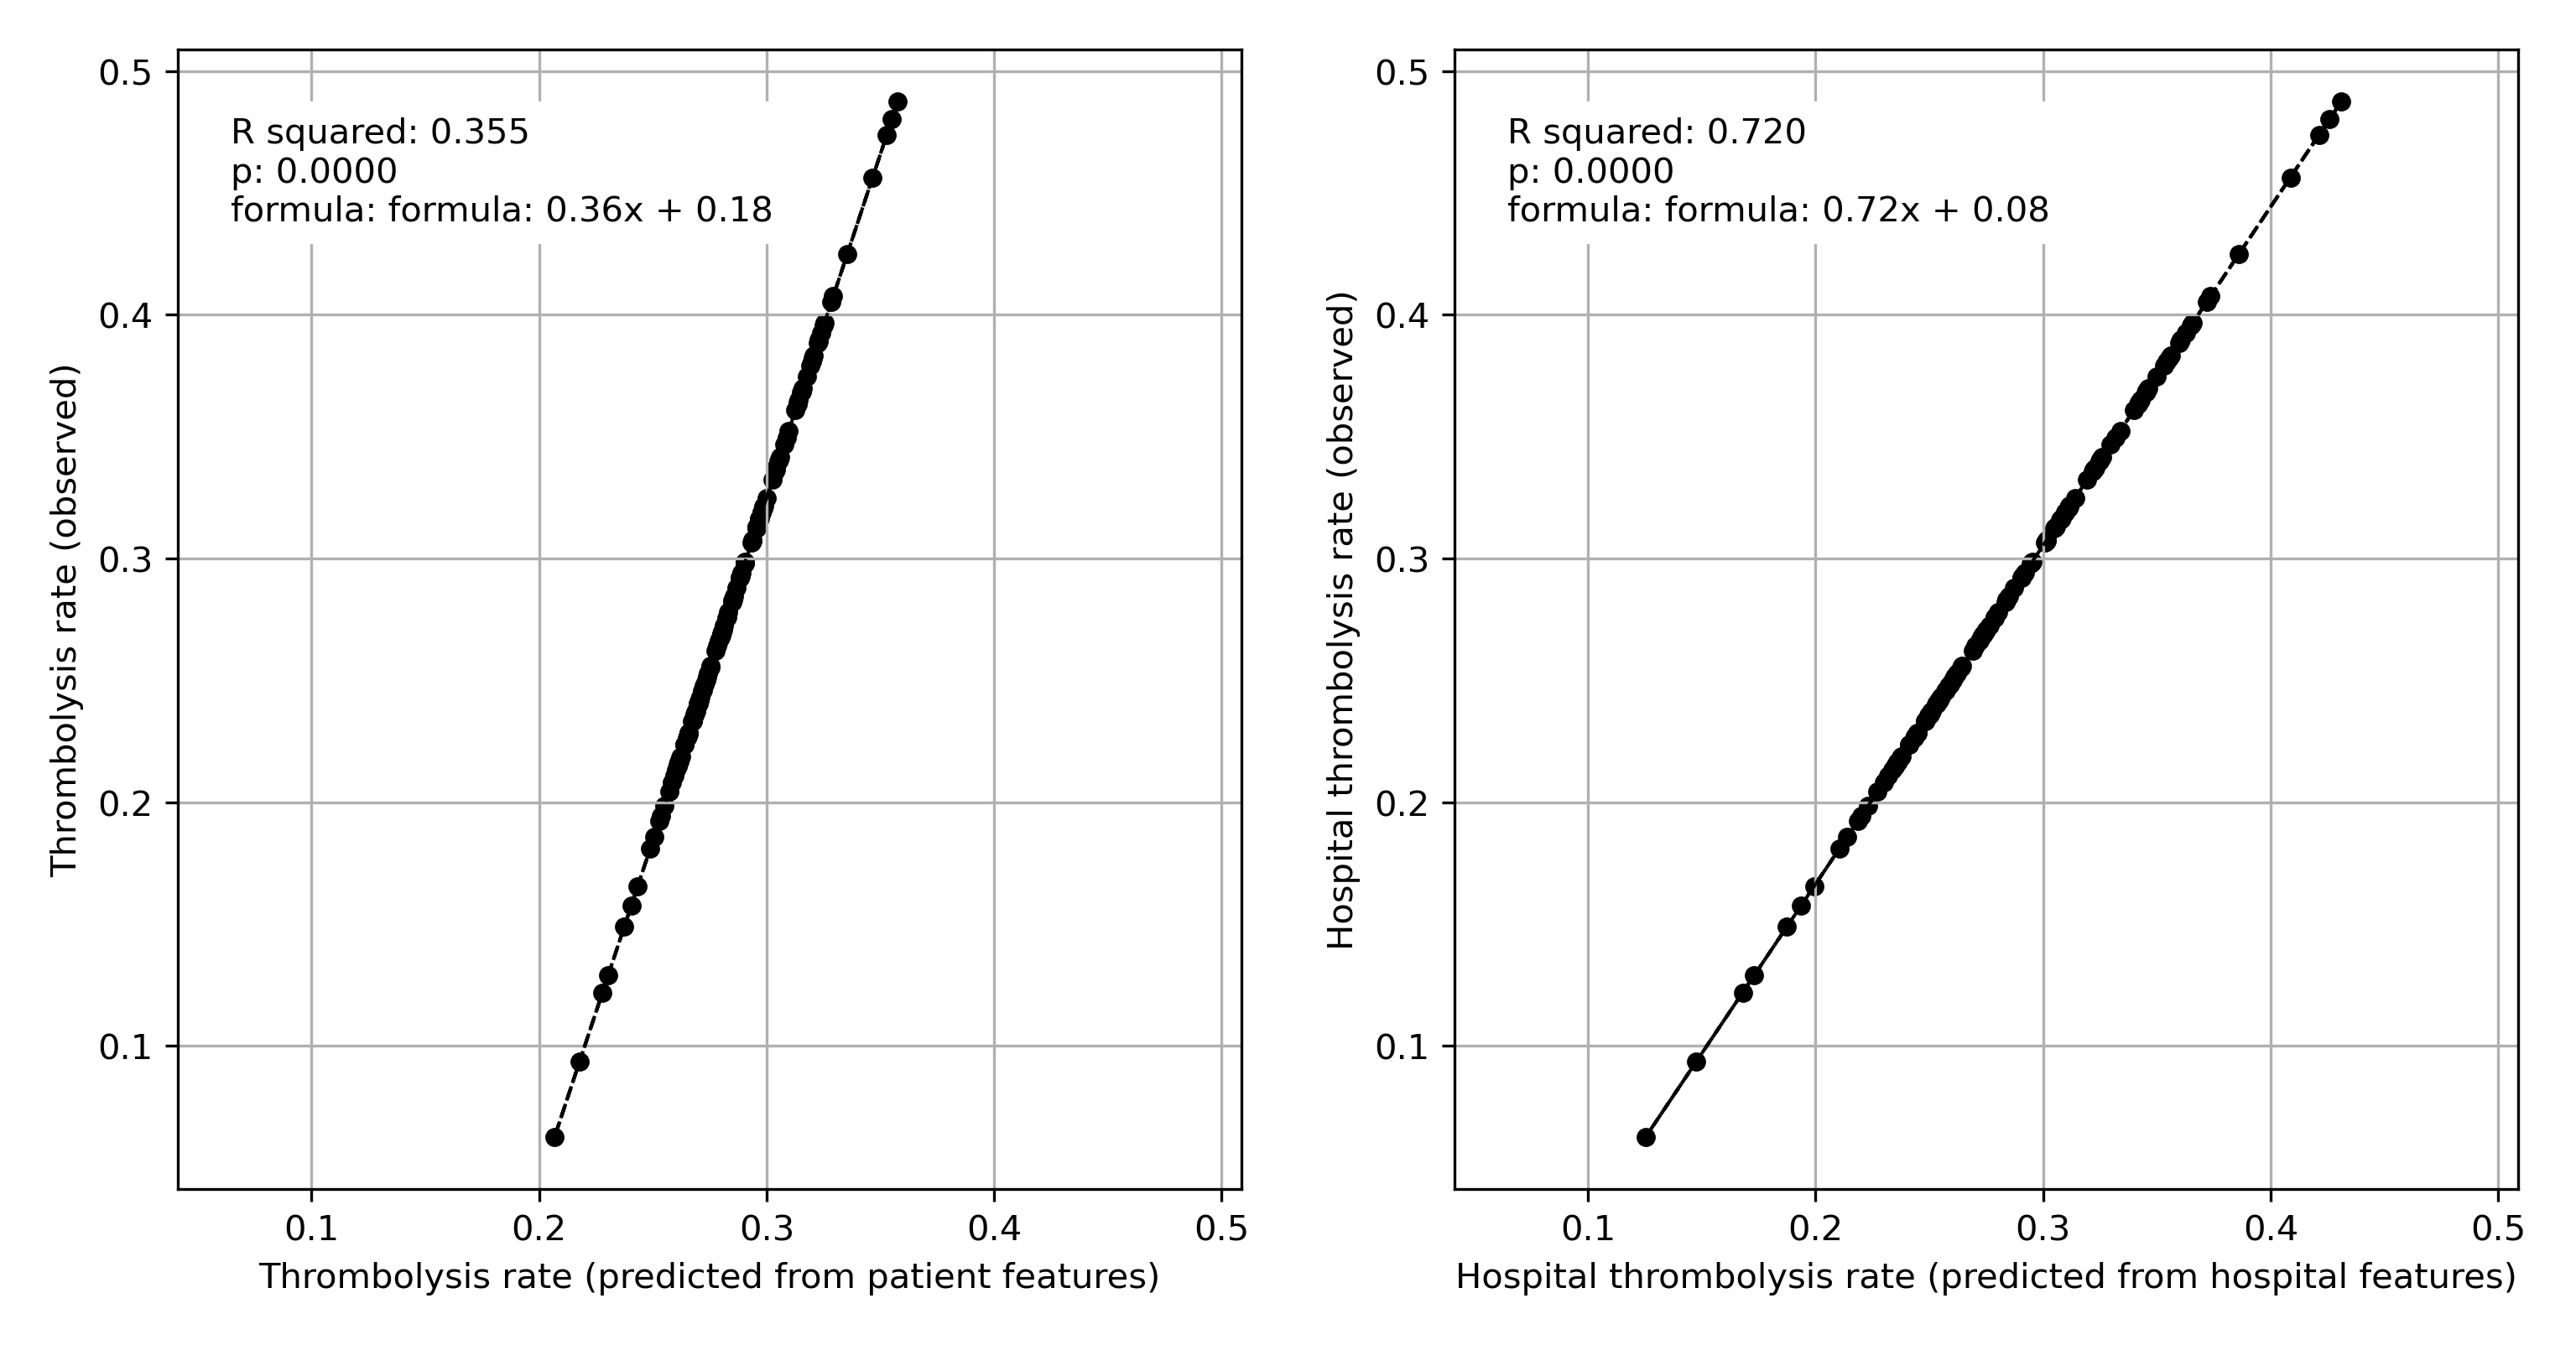
\includegraphics[width=0.9\textwidth]{./images/03e_xgb_10_features_multiple_regression_patient_hosptial}
    \caption{Multiple regression of revised SHAP values (median of patients attending hospital) with hospital observed thrombolyis rate. LHS: Revised SHAP values refined to the eight patient descriptive features (age, stroke severity, prior disability, onset-to-arrival time, stroke type, type of onset time, anticoagulants, and onset during sleep). Middle: Revised SHAP values refined to the two hospital descriptive features (arrival-to-scan time, and hospital attended). RHS: Revised SHAP values for all 10 features (for both hospital and patient descriptive features).}
  \label{fig:shap_multiple_regression}
\end{figure}

%%%%%%%%%%%%%%%%%%%%%%%%%%%%%%%%%%%%%%%%%%%%%%%%%%%%%%%%%%%%%%%%%%%%%%%%
%\newpage
\subsection{Variation in hospital thrombolysis use for patient subgroups}

Figure \ref{fig:results_boxplot} shows a boxplot of observed and predicted use of thrombolysis, broken down by subgroup. The nine subgroups of patients with one non-ideal feature (NIHSS $<$5, estimated stroke onset time, pre-stroke mRS $>2$) all had reduced thrombolysis use, and combining these non-ideal features reduced thrombolysis use further. The observed and predicted thrombolysis use show the same general results, but some small differences existed: 1) The use of thrombolysis in \emph{ideal} patients is a little lower in the observed vs predicted results (mean hospital thrombolysis use = 89\% vs 99\%), 2) The predicted results show a stronger effect of combining non-ideal features, 3) The observed thrombolysis rate shows higher between-hospital variation than the predicted thrombolysis rate. This may be partly explained by the observed thrombolysis rate being based on different patients at each hospital, but may also be partly explained by actual use of thrombolysis being slightly more variable than predicted thrombolysis use (which will follow general hospital patterns, and will not include, for example, between-clinician variation at each hospital).

For both the observed and predicted thrombolysis, subgroup thrombolysis use tended to reduce in parallel (r-squared 0.221 to 0.308 in observed thrombolysis use, and 0.445 to 0.621 in the predicted thrombolysis use). \kpFIXME{Calculate and use new values}

\begin{figure}[!h]
\centering
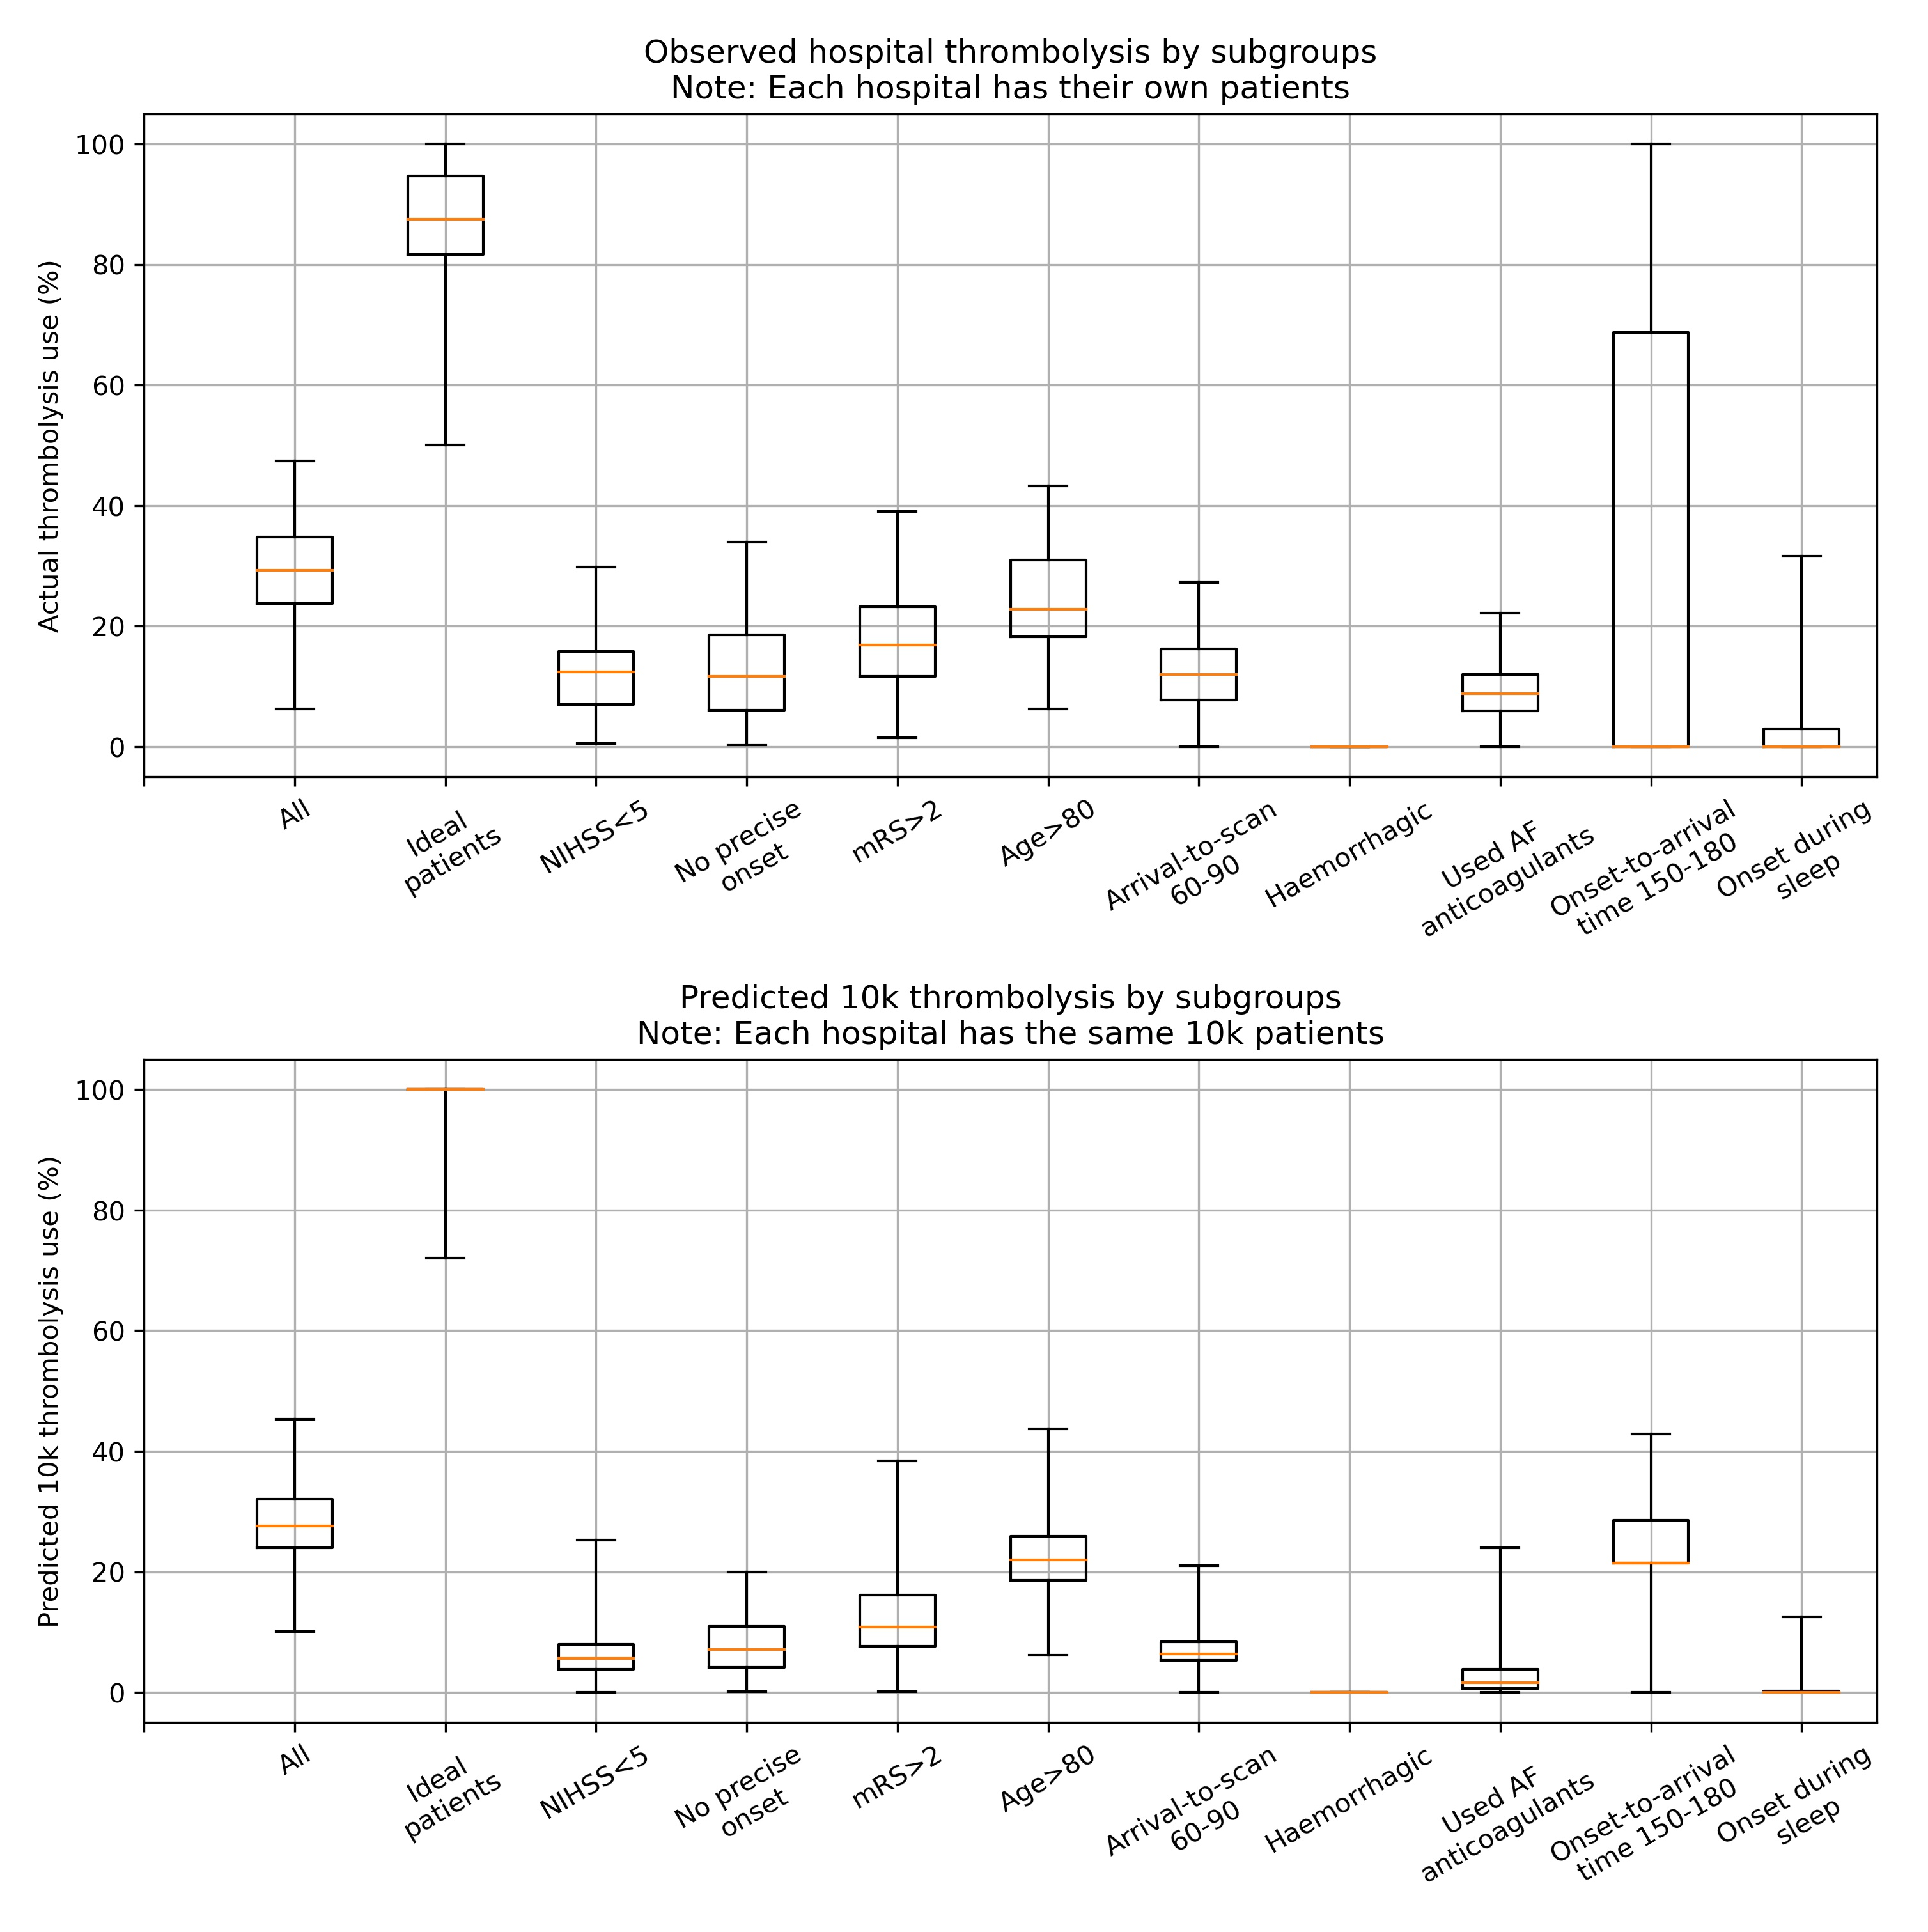
\includegraphics[width=1\textwidth]{./images/15a_xgb_10_features_10k_cohort_actual_vs_modelled_subgroup_violin}
%{./images/15a_actual_vs_modelled_subgroup_violin}
\caption{Boxplot for either observed (top) or predicted (bottom) use of thrombolysis for subgroups of patients.}
\label{fig:results_boxplot}
\end{figure}
\newpage





